\hypertarget{decksh-a-little-language-for-deck-markup}{%
\section{decksh: a little language for deck
markup}\label{decksh-a-little-language-for-deck-markup}}

\texttt{decksh} is a domain-specific language (DSL) for generating
\href{https://github.com/ajstarks/deck/blob/master/README.md}{\texttt{deck}}
markup.

\hypertarget{package-use}{%
\subsection{Package use}\label{package-use}}

There is a simple method \texttt{Process} that reads decksh commands
from an \texttt{io.Reader} and writes deck markup to an
\texttt{io.Writer}, returning an error.

\hypertarget{running}{%
\subsection{Running}\label{running}}

This repository also contains \texttt{cmd/decksh}, a client decksh
command:

\texttt{decksh} reads from the specified input, and writes deck markup
to the specified output destination:

\begin{verbatim}
$ decksh                   # input from stdin, output to stdout
$ decksh -o foo.xml        # input from stdin, output to foo.xml
$ decksh foo.sh            # input from foo.sh output to stdout
$ decksh -o foo.xml foo.sh # input from foo.sh output to foo.xml
\end{verbatim}

Typically, \texttt{decksh} acts as the head of a rendering pipeline:

\begin{verbatim}
$ decksh text.dsh | pdf -pagesize 1200,900 
\end{verbatim}

\hypertarget{example-input}{%
\subsection{Example input}\label{example-input}}

This deck script:

\begin{verbatim}
// Example deck
midx=50
midy=50
iw=640
ih=480

imfile="follow.jpg"
imlink="https://budnitzbicycles.com"
imscale=58
dtop=87

opts="-fulldeck=f -textsize 1  -xlabel=2  -barwidth 1.5"
deck
    slide "white" "black"
        ctext "Deck elements" midx dtop 5
        cimage "follow.jpg" "Dreams" 72 midy iw ih imscale imlink
        textblock "Budnitz #1, Plainfield, NJ, May 10, 2015" 55 35 10 1 "serif" "white"

        // List
        blist 10 75 3
            li "text, image, list"
            li "rect, ellipse, polygon"
            li "line, arc, curve"
        elist

        // Graphics
        gy=10
        c1="red"
        c2="blue"
        c3="green"
        rect    15 gy 8 6              c1
        ellipse 27.5 gy 8 6            c2
        polygon "37 37 45" "7 13 10"   c3
        line    50 gy 60 gy 0.25       c1
        arc     70 gy 10 8 0 180 0.25  c2
        curve   80 gy 95 25 90 gy 0.25 c3


        // Chart
        chartleft=10
        chartright=45
        charttop=42
        chartbottom=28
        dchart -left chartleft -right chartright -top charttop -bottom chartbottom opts AAPL.d 
    eslide
edeck
\end{verbatim}

Produces:

\begin{figure}
\centering
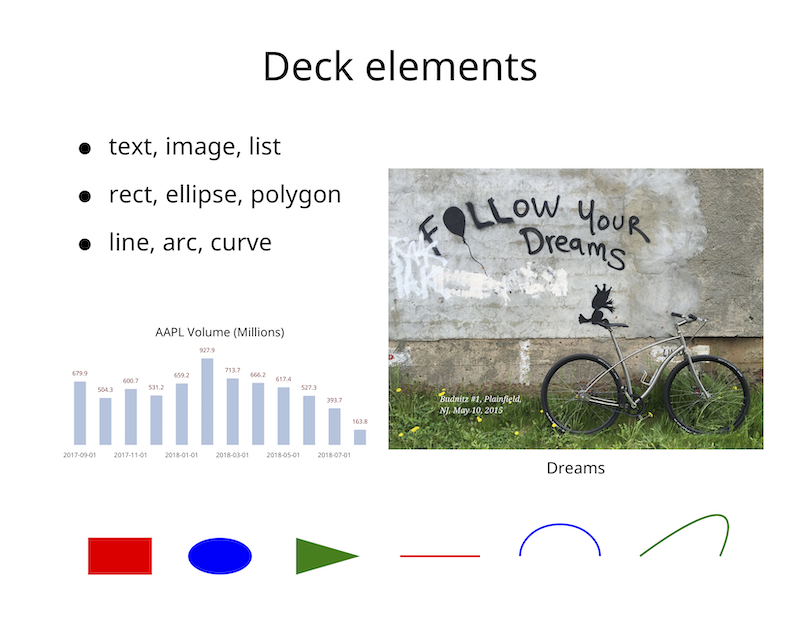
\includegraphics{exampledeck.png}
\caption{exampledeck}
\end{figure}

Text, font, color, caption and link arguments follow Go convetions
(surrounded by double quotes). Colors are in rgb format
(``rgb(n,n,n)''), hex (``\#rrggbb''), or
\href{https://www.w3.org/TR/SVG11/types.html\#ColorKeywords}{SVG color
names}.

Coordinates, dimensions, scales and opacities are floating point numbers
ranging from from 0-100 (they represent percentages on the canvas width
and percent opacity). Some arguments are optional, and if omitted
defaults are applied (black for text, gray for graphics, 100\% opacity).

Canvas size and image dimensions are in pixels.

\hypertarget{simple-assignments}{%
\subsection{Simple assignments}\label{simple-assignments}}

\texttt{id=\textless{}number\textgreater{}} defines a constant, which
may be then subtitited. For example:

\begin{verbatim}
x=10
y=20
text "hello, world" x y 5
\end{verbatim}

\hypertarget{assignment-operations}{%
\subsection{Assignment operations}\label{assignment-operations}}

\texttt{id+=\textless{}number\textgreater{}} increment the value of
\texttt{id} by \texttt{\textless{}number\textgreater{}}

\begin{verbatim}
x+=5
\end{verbatim}

\texttt{id-=\textless{}number\textgreater{}} decrement the value of
\texttt{id} by \texttt{\textless{}number\textgreater{}}

\begin{verbatim}
x-=10
\end{verbatim}

\texttt{id*=\textless{}number\textgreater{}} multiply the value of
\texttt{id} by \texttt{\textless{}number\textgreater{}}

\begin{verbatim}
x*=50
\end{verbatim}

\texttt{id*=\textless{}number\textgreater{}} divide the value of
\texttt{id} by \texttt{\textless{}number\textgreater{}}

\begin{verbatim}
x/=100
\end{verbatim}

\hypertarget{binary-operations}{%
\subsection{Binary operations}\label{binary-operations}}

Addition
\texttt{id=\textless{}id\textgreater{}\ +\ number\ or\ \textless{}id\textgreater{}}

\begin{verbatim}
tx=10
spacing=1.2

sx=tx-10
vx=tx+spacing
\end{verbatim}

Subtraction
\texttt{id=\textless{}id\textgreater{}\ -\ number\ or\ \textless{}id\textgreater{}}

\begin{verbatim}
a=x-10
\end{verbatim}

Muliplication
\texttt{id=\textless{}id\textgreater{}\ *\ number\ or\ \textless{}id\textgreater{}}

\begin{verbatim}
a=x*10
\end{verbatim}

Division
\texttt{id=\textless{}id\textgreater{}\ /\ number\ or\ \textless{}id\textgreater{}}

\begin{verbatim}
a=x/10
\end{verbatim}

\hypertarget{begin-or-end-a-deck.}{%
\subsection{Begin or end a deck.}\label{begin-or-end-a-deck.}}

\begin{verbatim}
deck
edeck
\end{verbatim}

\hypertarget{begin-end-a-slide-with-optional-background-and-text-colors.}{%
\subsection{Begin, end a slide with optional background and text
colors.}\label{begin-end-a-slide-with-optional-background-and-text-colors.}}

\begin{verbatim}
slide [bgcolor] [fgcolor]
eslide
\end{verbatim}

\hypertarget{specify-the-size-of-the-canvas.}{%
\subsection{Specify the size of the
canvas.}\label{specify-the-size-of-the-canvas.}}

\begin{verbatim}
canvas w h
\end{verbatim}

\hypertarget{random-number}{%
\subsection{Random Number}\label{random-number}}

\begin{verbatim}
x=random min max
\end{verbatim}

assign a random number in the specified range

\hypertarget{mapping}{%
\subsection{Mapping}\label{mapping}}

\begin{verbatim}
x=vmap v vmin vmax min max
\end{verbatim}

For value \texttt{v}, map the range \texttt{vmin-vmax} to
\texttt{min-max}.

\hypertarget{polar-coordinates}{%
\subsection{Polar Coordinates}\label{polar-coordinates}}

\begin{verbatim}
x=polarx cx cy r theta
y=polary cx cy r theta
\end{verbatim}

Return the polar coordinate given a center at \texttt{(cx,\ cy)}, radius
\texttt{r}, and angle \texttt{theta} (in degrees)

\hypertarget{area}{%
\subsection{Area}\label{area}}

\begin{verbatim}
a=area d
\end{verbatim}

return the circular area, \texttt{a} for the diameter \texttt{d}.

\hypertarget{formatted-text}{%
\subsection{Formatted Text}\label{formatted-text}}

Assign a string variable with formatted text (using package fmt floating
point format strings)

\begin{verbatim}
w1=10
w2=20+100

s0=format "Widget 1: %.2f" w1
s1=format "Widget 2: %.3f" w2
st=format "Total Widgets: %v" s1+w2
\end{verbatim}

\hypertarget{loops}{%
\subsection{Loops}\label{loops}}

Loop over \texttt{statements}, with \texttt{x} starting at
\texttt{begin}, ending at \texttt{end} with an optional
\texttt{increment} (if omitted the increment is 1). Substitution of
\texttt{x} will occur in statements.

\begin{verbatim}
for x=begin end [increment]
    statements
efor
\end{verbatim}

Loop over \texttt{statements}, with \texttt{x} ranging over the contents
of items within \texttt{{[}{]}}. Substitution of \texttt{x} will occur
in statements.

\begin{verbatim}
for x=["abc" "def" "ghi"]
    statements
efor
\end{verbatim}

Loop over \texttt{statements}, with \texttt{x} ranging over the contents
\texttt{"file"}. Substitution of \texttt{x} will occur in statements.

\begin{verbatim}
for x="file"
    statements
efor
\end{verbatim}

\hypertarget{text}{%
\subsection{Text}\label{text}}

Left, centered, end, or block-aligned text (\texttt{x} and \texttt{y}
are the text's reference point), or a file's contents with optional font
(``sans'', ``serif'', ``mono'', or ``symbol''), color and opacity.

\begin{verbatim}
text       "text"     x y size       [font] [color] [opacity] [link]
ctext      "text"     x y size       [font] [color] [opacity] [link]
etext      "text"     x y size       [font] [color] [opacity] [link]
textblock  "text"     x y width size [font] [color] [opacity] [link]
\end{verbatim}

Text rotated along the specified angle (in degrees)

\begin{verbatim}
rtext      "text"     x y angle size [font] [color] [opacity] [link]
\end{verbatim}

Text on an arc centered at \texttt{(x,y)}, with specified radius,
between begin and ending angles (in degrees). if the beginning angle is
less than the ending angle the text is rendered counter-clockwise. if
the beginning angle is greater than the ending angle, the text is
rendered clockwise.

\begin{verbatim}
arctext    "text"     x y radius begin-angle end-angle size [font] [color] [opacity] [link]
\end{verbatim}

Place the contents of ``filename'' at (x,y). Place the contents of
``filename'' in gray box, using a monospaced font.

\begin{verbatim}
textfile   "filename" x y       size [font] [color] [opacity] [linespacing]
textcode   "filename" x y width size [color]
\end{verbatim}

\hypertarget{images}{%
\subsection{Images}\label{images}}

Plain and captioned, with optional scales, links and caption size.
\texttt{(x,\ y)} is the center of the image, and \texttt{width} and
\texttt{height} are the image dimensions in pixels.

\begin{verbatim}
image  "file"           x y width height [scale] [link]
cimage "file" "caption" x y width height [scale] [link] [size]
\end{verbatim}

\hypertarget{lists}{%
\subsection{Lists}\label{lists}}

(plain, bulleted, numbered, centered). Optional arguments specify the
color, opacity, line spacing, link and rotation (degrees)

\begin{verbatim}
list   x y size [font] [color] [opacity] [linespacing] [link] [rotation]
blist  x y size [font] [color] [opacity] [linespacing] [link] [rotation]
nlist  x y size [font] [color] [opacity] [linespacing] [link] [rotation]
clist  x y size [font] [color] [opacity] [linespacing] [link] [rotation]
\end{verbatim}

\hypertarget{list-items-and-ending-the-list}{%
\subsubsection{list items, and ending the
list}\label{list-items-and-ending-the-list}}

\begin{verbatim}
li "text"
elist
\end{verbatim}

\hypertarget{graphics}{%
\subsection{Graphics}\label{graphics}}

Rectangles, ellipses, squares, circles: specify the center location
\texttt{(x,\ y)} and dimensions \texttt{(w,h)} with optional color and
opacity. The default color and opacity is gray, 100\%. In the case of
the \texttt{acircle} keyword, the \texttt{a} argument is the area, not
the diameter.

\begin{verbatim}
rect    x y w h [color] [opacity]
ellipse x y w h [color] [opacity]

square  x y w   [color] [opacity]
circle  x y w   [color] [opacity]
acircle x y a   [color] [opacity]
\end{verbatim}

Rounded rectangles are similar, with the added radius for the corners:
(solid colors only)

\begin{verbatim}
rrect   x y w h r [color]
\end{verbatim}

For polygons, specify the x and y coordinates as a series of numbers,
with optional color and opacity.

\begin{verbatim}
polygon "xcoords" "ycoords" [color] [opacity]
\end{verbatim}

Note that the coordinates may be either discrete:

\begin{verbatim}
polygon "10 20 30" "50 60 50"
\end{verbatim}

or use substitution:

\begin{verbatim}
x1=10
x2=20
x3=30
y1=50
y2=y1+10
y3=y1
polygon "x1 x2 x3" "y1 y2 y3"
\end{verbatim}

A combination of constants and substitution is also allowed.

\begin{verbatim}
polygon "20 x2 30" "50 y2 50"
\end{verbatim}

For lines, specify the coordinates for the beginning \texttt{(x1,y1)}
and end points \texttt{(x2,\ y2)}. For horizontal and vertical lines
specify the initial point and the length. Line thickness, color and
opacity are optional, with defaults (0.2, gray, 100\%).

A ``pill'' shape has is a horizontal line with rounded ends.

\begin{verbatim}
line    x1 y1 x2 y2 [size] [color] [opacity]
hline   x y length  [size] [color] [opacity]
vline   x y length  [size] [color] [opacity]
pill    x w length  size   [color]
\end{verbatim}

Curve is a quadratic Bezier curve: specify the beginning location
\texttt{(bx,\ by)}, the control point \texttt{(cx,\ cy)}, and ending
location \texttt{(ex,\ ey)}.

For arcs, specify the location of the center point \texttt{(x,y)}, the
width and height, and the beginning and ending angles (in degrees). Line
thickness, color and opacity are optional, with defaults (0.2, gray,
100\%).

\begin{verbatim}
curve   bx by cx cy ex ey [size] [color] [opacity]
arc     x y w h a1 a2     [size] [color] [opacity]
\end{verbatim}

To make n-sided stars, use the ``star'' keyword: \texttt{(x,y)} is the
center of the star, \texttt{np} is the number of points, and
\texttt{inner} and \texttt{outer} are the sizes of the inner and outer
points, respectively.

\begin{verbatim}
star    x y np inner outer [color] [opacity]
\end{verbatim}

\hypertarget{arrows}{%
\subsection{Arrows}\label{arrows}}

Arrows with optional linewidth, width, height, color, and opacity.
Default linewidth is 0.2, default arrow width and height is 3, default
color and opacity is gray, 100\%. The curve variants use the same syntax
for specifying curves.

\begin{verbatim}
arrow   x1 y1 x2 y2       [linewidth] [arrowidth] [arrowheight] [color] [opacity]
lcarrow bx by cx cy ex ey [linewidth] [arrowidth] [arrowheight] [color] [opacity]
rcarrow bx by cx cy ex ey [linewidth] [arrowidth] [arrowheight] [color] [opacity]
ucarrow bx by cx cy ex ey [linewidth] [arrowidth] [arrowheight] [color] [opacity]
dcarrow bx by cx cy ex ey [linewidth] [arrowidth] [arrowheight] [color] [opacity]
\end{verbatim}

\hypertarget{braces}{%
\subsection{Braces}\label{braces}}

Left, right, up and down-facing braces. (x, y) is the location of the
point of the brace, and linewidth, color and opacity are optional
(defaults are gray, 100\%)

\begin{verbatim}
lbrace x y height aw ah [linewidth] [color] [opacity]
rbrace x y height aw ah [linewidth] [color] [opacity]
ubrace x y width  aw ah [linewidth] [color] [opacity]
dbrace x y width  aw ah [linewidth] [color] [opacity]
\end{verbatim}

\hypertarget{charts}{%
\subsection{Charts}\label{charts}}

Run the
\href{https://github.com/ajstarks/dchart/blob/master/README.md}{dchart}
command with the specified arguments.

\begin{verbatim}
dchart [args]
\end{verbatim}

\hypertarget{legend}{%
\subsection{Legend}\label{legend}}

Show a colored legend

\begin{verbatim}
legend "text" x y size [font] [color]
\end{verbatim}

\hypertarget{include-decksh-markup-from-a-file}{%
\subsection{Include decksh markup from a
file}\label{include-decksh-markup-from-a-file}}

\begin{verbatim}
include "file"
\end{verbatim}

places the contents of \texttt{"file"} inline.

\hypertarget{data-make-a-file}{%
\subsection{Data: Make a file}\label{data-make-a-file}}

\begin{verbatim}
data "foo.d"
uno    100
dos    200
tres   300
edata
\end{verbatim}

makes a file named \texttt{foo.d} with the lines between \texttt{data}
and \texttt{edata}.

\hypertarget{grid-place-objects-on-a-grid}{%
\subsection{Grid: Place objects on a
grid}\label{grid-place-objects-on-a-grid}}

\begin{verbatim}
grid "file.dsh" x y xskip yskip limit
\end{verbatim}

The first file argument (\texttt{"file.dsh"} above) specifies a file
with decksh commands; each item in the file must include the arguments
``x'' and ``y''. Normal variable substitution occurs for other
arguments. For example if the contents of \texttt{file.dsh} has six
items:

\begin{verbatim}
circle x y 5
circle x y 10
circle x y 15
square x y 5
square x y 10
square x y 15
\end{verbatim}

The line:

\begin{verbatim}
grid "file.dsh" 10 80 20 30 50
\end{verbatim}

creates two rows: three circles and then three squares

\texttt{x,\ y} specify the beginning location of the items,
\texttt{xskip} is the horizontal spacing between items.
\texttt{yinternal} is the vertical spacing between items and
\texttt{limit} the the horizontal limit. When the \texttt{limit} is
reached, a new row is created.
